\section[Motivation]{Motivation}
\begin{frame}
  \frametitle{Motivation}
  \begin{columns}
    \begin{column}{0.5\textwidth}
      \begin{block}{Why polymer solutions?}
        \begin{itemize}
        \item Turbulent drag reduction
        \item Elastic instabilities and elastic turbulence leads to efficient mixing in microchannel flow
        \end{itemize}
      \end{block}
      \begin{block}{Why SDPD?}
        \begin{itemize} 
        \item Direct presentation of conformation of polymer molecules
        \item Easy measurement of elastic stress field
        \end{itemize}
      \end{block}

    \end{column}
    \begin{column}{0.5\textwidth}
\begin{figure}[t]
    \centering
    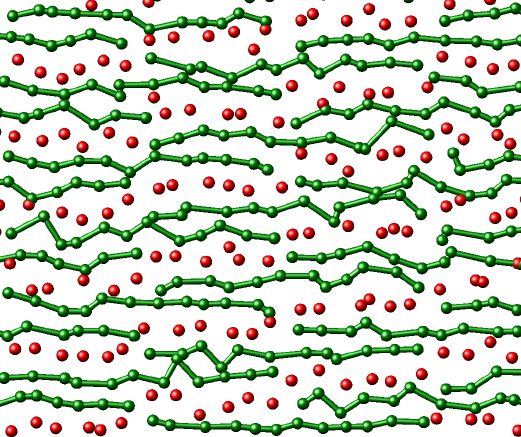
\includegraphics[width=0.6\textwidth]{img/polymers.png}
    \caption{Snapshot of polymer solutions in 2D.}
    \label{fig:snap}
  \end{figure}
    \end{column}
  \end{columns}
%   \footnotetext{\tiny \bibentry{baldassari2012flow}}
\end{frame}

\begin{frame}
  \frametitle{Motivation II}

  \begin{block}{Why Four-Roll Mill Flow?}
    \begin{itemize}
    \item Extensional flow is more effective to locally 
          stretch polymer molecules than simple shear flow
\item Polymer molecules are strongly stretched at extensional points in a micro-channel cross flow
    \end{itemize}

  \end{block}
The four-roll mill flow is driven by a steady background force in 2D:
\begin{equation}
\mathbf{F}=\left\{\begin{matrix}
C_0sin(\frac{2\pi x} {L})cos(\frac{2\pi x} {L})
\\ 
-C_0cos(\frac{2\pi x} {L})sin(\frac{2\pi x} {L})
\end{matrix}\right.
\end{equation}
%   \begin{block}{Viscosity}
%     $1<\text{Re}<2000$ $\implies$ full Navier-Stokes (NS) equations~\footnotemark
%   \end{block}
%   \footnotetext{\tiny \bibentry{worner_numerical_2012}}
\end{frame}

\begin{frame}
  \frametitle{Related Work}
\begin{block}{Numerical Simulation by Thomases et al. with DNS~\footnotemark: }
\begin{itemize}
 \item Beyond a first critical Wi number, the flow near the stagnation point becomes asymmetric and stretched.
\item At higher Wi number, the flow is dominated by a single large vortex and persistent oscillations occur. 
\end{itemize}
\end{block}
\begin{block}{Experiments by Liu et al.~\footnotemark[2]:}
\begin{itemize}
 \item  At low Wi the flow pattern is nearly Newtonian. 
\item At higher Wi, the strength and the position of the vortices fluctuates periodically.
\item At even higher Wi, the flow field fluctuates stochastically in space and time.
\end{itemize}
\end{block}
\footnotetext{\tiny \bibentry{Thomases2011}}
\footnotetext[2]{\tiny \bibentry{Liu2012}}
\end{frame}

% \begin{frame}
%   \frametitle{Models}
%   \begin{itemize}
%   \item VOF \\
%     \bibintext{welch_local_1995}, \\
%     \bibintext{kunkelmann_cfd_2009}
%   \item Lattice Boltzmann \\
%     \bibintext{markus_pool_2012}
%   \item Particle-Based \\
%     \bibintext{muller_particle-based_2005}, \\ 
%    \bibintext{yoon_direct_2001}
%   \end{itemize}
% \end{frame}

%%% Local Variables: 
%%% mode: latex
%%% TeX-master: t
%%% End: 
